\documentclass[a4paper,10pt]{article}

\usepackage[english]{babel}
\usepackage{graphicx}
\usepackage[colorlinks, allcolors=black]{hyperref}
\usepackage{geometry}
\geometry{tmargin=3cm, bmargin=2.2cm, lmargin=2.2cm, rmargin=2cm}
\usepackage{todonotes} %Used for the figure placeholders
\usepackage[space]{grffile}

% Your name and student number must be filled in on the title page found in
% titlepage.tex.

\begin{document}
\begin{titlepage}
    \newpage
    \thispagestyle{empty}
    \frenchspacing
    \hspace{-0.2cm}
    
\includegraphics[height=3.4cm]{sedes}
    \hspace{0.2cm}
    \rule{0.5pt}{3.4cm}
    \hspace{0.2cm}
    \begin{minipage}[b]{8cm}
        \Large{Katholieke\newline Universiteit\newline Leuven}\smallskip\newline
        \large{}\smallskip\newline
        \textbf{Department of\newline Computer Science}\smallskip
    \end{minipage}
    \hspace{\stretch{1}}
    \vspace*{3.2cm}\vfill
    \begin{center}
        \begin{minipage}[t]{\textwidth}
            \begin{center}
                \LARGE{\rm{\textbf{\uppercase{Document Processing}}\\The
                complete architecture}}\\
                \Large{\rm{Software Architecture (H09B5a and H07Z9a) -- 
                Part 2b}}
            \end{center}
        \end{minipage}
    \end{center}
    \vfill
    \hfill\makebox[8.5cm][l]{%
        \vbox to 7cm{\vfill\noindent
            {\rm \textbf{Thomas Vochten (r0300128)}}\\
            {\rm \textbf{Frederik Goovaerts (r0256551)}}\\[2mm]
            {\rm Academic year 2014--2015}
        }
    }
\end{titlepage}


\tableofcontents
\newpage

\section{Introduction}\label{sec:introduction}

The goal of this project was to design an architecture for a Document Processing system. Companies can use this system to submit data for payslips and invoices, and the corresponding documents are generated and delivered for them. This way, they do not have to provide the infrastructure for this themselves. The architecture as developed and explained in the following sections conforms to the functional and non-functional requirements as imposed by the assignment.

\section{Overview}\label{sec:overview}
\subsection{Architectural decisions}

\paragraph{Av1a and Av2a\@: notification of the eDocs Administrator}
\emph{Av1a} and \emph{Av2a} expect a system for notifying the eDocs Administrator of errors within 1 minute. For this purpose, there is a \texttt{Communication Subsystem}, capable of swiftly relaying Error Notifications to the eDocs Administrator. The \texttt{Subsystem} is also responsible for relaying normal message (non-internal errors, standard email deliveries etc.), but this responsibility can be inhibited if system errors are reported, so they take precedence.\\
\emph{Employed tactics and patterns: None}
    
\paragraph{Av1b\@: storing the status of an individual job}
A general \texttt{Job Storage Subsystem} is introduced to the system, to store among others the status of all jobs. For \emph{Av1b}, the \texttt{GeneratorManager} has access to this \texttt{Subsystem}, to change the status of a failed job to ``Temporarily failed''.\\
\emph{Employed tactics and patterns: None}
    
\paragraph{Av2b\@: temporary storage of Personal Document Store documents} \emph{Av2b} specifies that the system should be able to temporarily store three hours of documents should the Personal Document Store fail and furthermore that a maximally functional user interface that clearly indicates that the Personal Document Store is down should be presented. To tackle the first of these requirements, we institute a \texttt{PDSCache} in the \texttt{DocumentStorageHandler} (which is a subcomponent of the \texttt{DocumentDB}, in turn). To fulfil the second, the \texttt{LookupSubsystem} keeps pinging the \texttt{PDSDB}, answering any lookup queries with a message that the Personal Document Store is not available until the ping succeeds. For more details, we refer to section \todo{Av2b label}\\
\emph{Employed tactics and patterns: buffer, ping.}
    
\paragraph{Av3\@: Zoomit failure} \emph{Av3} specifies (1) that the system should be able to detect when an invoice is not accepted by Zoomit (2) that the system should retry several times before taking other measures (3) notify the eDocs administrators of this failure and (4) store at least two days of documents to be delivered via Zoomit. To handle (1) and (2), the \texttt{ZoomitDeliveryHandler} should be implemented appropriately. In order to fulfil (3), the \texttt{ZoomitDeliveryHandler} has access to messaging facilities in the \texttt{CommunicationSubsystem}. To tackle (4), the \texttt{ZoomitDocumentLinkCache} is introduced that stores \texttt{JobID}s of documents to be delivered via Zoomit. For more details, we refer to section \todo{Av3 label}\\
\emph{Employed tactics and patterns: buffer.}
    
\paragraph{P2\@: document lookups}
For handling Document Lookups in a timely fashion, a \texttt{Lookup Subsystem} has been introduced to the system. This \texttt{Subsystem} handles both PDS and Download lookups, monitoring the amount of requests for both sides. When one side is in danger performance-wise because of the other, the \texttt{Subsystem} will throttle the overactive side, so the system keeps performing as expected for both Download and PDS lookups. Enough redundancy in the form of \emph{active replication} is provided in the \texttt{Storage Subsystem} such that lookups and storage of generated documents can be executed simultaneously without having a large impact upon one another.\\
\emph{Employed tactics and patterns: Active replication, Manage event rate}
    
\paragraph{P3\@: status overview for Customer Administrators} \emph{P3} specifies that Customer Administrators should be able to retrieve the status of all documents in a timely fashion. Furthermore, retrieval of this status should have as low an impact as possible on the rest of the system. In view of this, the \texttt{JobStorageSubsystem} has a subcomponent dedicated to storing the status of all jobs, the \texttt{JobStatusDatabase}. In this database, we have applied active replication in order to speed up any reads. \emph{P3} requires that the resulting view be consistent up to one minute ago; we assume that active replication is no obstacle to that. For more details, we refer to section \todo{P3 label}\\
\emph{Employed tactics and patterns: Increase available resources, active replication.}
    
\paragraph{M1\@: New type of document - bank statements} \emph{M1} requires that the addition of bank statements as new document type to the system be as convenient as possible. The most important consideration is that the system should support specifying new templates for the new document type, since generation consists of filling out the fields contained in the template. In other parts of the system, we ensured that behaviour is not coupled too tightly to the type of a specific document. For more details, we refer to section \todo{M1 label}\\
\emph{Employed tactics and patterns: Hide information, generalize module.}
    
\paragraph{M2\@: Multiple print \& postal services} 
In the \texttt{Delivery Subsystem}, the different delivery channels are viewed as black boxes for delivery. They manage their own delivery, billing and job status management where necessary. The delivery channel for postal delivery is the only part of the system to be modified for this requirement. The delivery channel could have a set of possible PPS companies of which to select the desired one. The selection of the desired company could be an extra field in the delivery metadata, while no extra information warrants the default PPS company.\\
\emph{Employed tactics and patterns: Maintain existing interface, Abstract common services}
    
\paragraph{M3\@: Dynamic selection of the cheapest of print \& postal services}
Cfr. \emph{M2}, the postal delivery channel can be modified without changing the rest of the system. This delivery channel can then internally analyse the cost for the delivery of a document, based on the delivery address and set of PPS companies available.\\
\emph{Employed tactics and patterns: Abstract common services}

\subsection{Discussion}
Use this section to discuss your architecture in retrospect.
For example, what are the strong points of your architecture?
What are the weak points? Is there anything you would have done otherwise with
your current experience?
Are there any remarks about the architecture that you would give to your
customers?
Etc.

\section{Client-server view (UML Component diagram)}\label{sec:client-server}
The context diagram of the client-server view.
Discuss which components communicate with external components and what these
external components represent.

\begin{figure}[!htp]
    \centering
    %\includegraphics[width=\textwidth]{}
    \missingfigure[figwidth=0.8\textwidth]{Context diagram of the client-server
        view.}
    \caption{Context diagram for the client-server view.
        }\label{fig:cc-context}
\end{figure}

The primary diagram and accompanying explanation.

\begin{figure}[!htp]
    \centering
    %\includegraphics[width=\textwidth]{}
    \missingfigure[figwidth=0.8\textwidth]{Primary diagram of the client-server
        view.}
    \caption{Primary diagram of the client-server view.}\label{fig:cs-primary}
\end{figure}

\subsection{Main architectural decisions}
Discuss your architectural decisions for the most important requirements in
more detail using the components of the client-server view.
Pay attention to the solutions that you employed and the alternatives that you
considered.
The explanation here must be self-contained and complete.
Imagine you had to describe how the architecture supports the core
functionality to someone that is looking at the client-server view only.
Hide unnecessary details (these should be shown in the decomposition view).

\subsubsection{ReqX\@: requirement name}
Describe the design choices related to \emph{ReqX} together with the rationale
of why these choices where made.

\subsubsection*{Alternatives considered}
\paragraph{Alternative(s) for choice 1} Explain what alternative(s) you
considered for this design choice and why they where not selected.

\section{Decomposition view (UML Component diagram)}\label{sec:decomposition}
Discuss the decompositions of the components of the client-server view which
you have further decomposed.

\subsection{ComponentX}
\begin{figure}[!htp]
    \centering
    %\includegraphics[width=\textwidth]{}
    \missingfigure[figwidth=0.8\textwidth]{Diagram showing decomposition of
        ComponentX}
    \caption{Decomposition of \texttt{ComponentX}}\label{fig:decomp-componentx}
\end{figure}

Describe the decomposition of \texttt{ComponentX} and how this relates to the
requirements.

\section{Deployment view (UML Deployment diagram)}\label{sec:deployment}
Describe the context diagram for the deployment view.
For example, which protocols are used for communication with external systems
and why?

\begin{figure}[!htp]
    \centering
    %\includegraphics[width=\textwidth]{}
    \missingfigure[figwidth=0.8\textwidth]{Context diagram for the deployment
        view.}
    \caption{Context diagram for the deployment view.}\label{fig:depl_context}
\end{figure}

The primary deployment diagram itself and accompanying explanation.
Pay attention to the parts of the deployment diagram which are crucial for
achieving certain non-functional requirements.
Also discuss any alternative deployments that you considered.

\begin{figure}[!htp]
    \centering
    %\includegraphics[width=\textwidth]{}
    \missingfigure[figwidth=0.8\textwidth]{Primary diagram for the deployment
        view.}
    \caption{Primary diagram for the deployment view.}\label{fig:depl_primary}
\end{figure}

\section{Scenarios}\label{sec:scenarios}
Illustrate how your architecture fulfills the most important data flows.
As a rule of thumb, focus on the scenario of the domain description.
Describe the scenario in terms of architectural components using UML Sequence
diagrams and further explain the most important interactions in text.
Illustrating the scenarios serves as a quick validation of the completeness of
your architecture.
If you notice at this point that for some reason, certain functionality or
qualities are not addressed sufficiently in your architecture, it suffices to
document this, together with a rationale of why this is the case according to
you.
You do not have to further refine you architecture at this point.

\subsection{Scenario 1}
Shortly describe the scenario shown in this subsection.
Show the complete scenario using one or more sequence diagrams.

\begin{figure}[!htp]
    \centering
    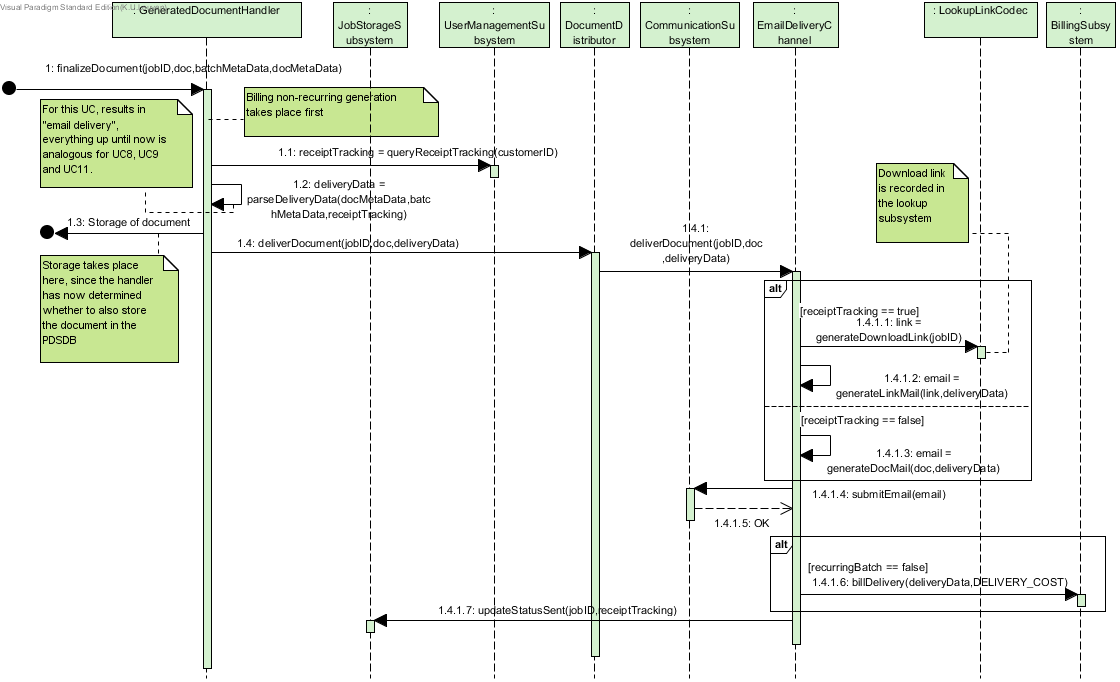
\includegraphics[width=\textwidth]{figures/UC6 - Deliver document via e-mail.png}
    %\missingfigure[figwidth=0.8\textwidth]{Sequence diagram scenario 1}
    \caption{The system behavior for the first scenario.
        }\label{fig:seq_scenario1}
\end{figure}

\appendix
\section{Element catalog}\label{app:catalog}
List all components and describe their responsibilities and provided
interfaces.
Per interface, list all methods using a Java-like syntax and describe their
effect and exceptions if any.
List all elements and interfaces alphabetically for ease of navigation.

\subsection{Component 1}
\begin{itemize}
    \item \textbf{Description:} Responsibilities of the component.
    \item \textbf{Super-component:} The direct super-component, if any.
    \item \textbf{Sub-components:} the direct sub-components, if any.
\end{itemize}

\subsubsection*{Provided interfaces}
\begin{itemize}
    \item InterfaceA
    \begin{itemize}
        \item \texttt{returntType1 operation1(ParamType param) throws SomeException}
        \begin{itemize}
            \item Effect: Describe the effect of the operation
            \item Exceptions:
            \begin{itemize}
                \item SomeException: Describe when the exception is thrown.
            \end{itemize}

            \item \texttt{void operation2(ParamType2 param)}
            \begin{itemize}
                \item Effect: Describe the effect of the operation
                \item Exceptions: None
            \end{itemize}
        \end{itemize}
    \end{itemize}

    \item InterfaceB
    \begin{itemize}
        \item \texttt{returntType2 operation3()}
        \begin{itemize}
            \item Effect: Describe the effect of the operation
            \item Exceptions: None
        \end{itemize}
    \end{itemize}
\end{itemize}

\section{Defined data types}\label{app:datatypes}
List and describe all data types defined in your interface specifications. List
them alphabetically for ease of navigation.

\begin{itemize}
	\item \texttt{DeliveryMetaData}: Contains the delivery channel, recipient address and other required delivery information (e.g. Customer Organization name, whether receipt tracking applies and whether it is from a recurring batch) for an individual document.
	\item \texttt{BatchDetails}: Encapsulates details about the batch a Customer Organization intends to upload (e.g. type of documents contained in the batch).
	\item \texttt{BatchMetaData}: Contains information such as the CustomerID, the document type of the batch and when it was received.
	\item \texttt{CustomerOrganizationID}: Corresponds to a certain Customer Organization.
	\item \texttt{Document}: Represents a generated document
	\item \texttt{DownloadLink}: Encoded link which decodes to a JobID.
	\item \texttt{GenerationErrorReport}: Contains information about the document for which generation failed (e.g. CustomerOrganizationID) and the reason for the error.
	\item \texttt{Job}: Encapsulates a RawDataEntry, together with its JobID and BatchID.
	\item \texttt{JobID}: Corresponds to a Job and later the Document generated from it.
	\item \texttt{JobStatusEntry}: Encapsulates document state concerning whether it has been generated, delivered, etc. and relevant time stamps.
    \item \texttt{LoginCredentials}: Used when the user wants to log in. Contains the username, password, function the user wants to log in as and general info about the user attempting the login (e.g. IP address).
    \item \texttt{LoginToken}: Depending on the type of user, authorises the user to perform certain actions within the system.
    \item \texttt{PDSLookupLink}: Encoded link which decodes to a JobID and RecipientID.
    \item \texttt{RawDataBatch}: Contains several RawDataEntries and an indication whether it concerns a recurring batch. 
    \item \texttt{RawDataEntry}: Contains all raw data and meta data necessary such that a document can be generated.
    \item \texttt{RawDataMetaData}: Contains information such as the identifier of the raw data unique within the Customer Organization, the selected delivery channel, the name of the addressee and the address of the addressee (the form of which depends on the selected delivery channel).
    \item \texttt{RegistrationDetails}: Contains details that can be used to register a Recipient such as first name, last name, e-mail address and postal address.
    \item \texttt{Template}: Contains fields that can be filled out and an indication which fields are mandatory.
    \item \texttt{UserSession}: Container for login token; keeps state for logged-in user.
\end{itemize}

\end{document}
